\section{Additional Generalization Diagnostics}

Figure~\ref{fig:appendix-gap} examines two generalization diagnostics using the same peptide-pair pools as the fourth research question. The upper panel reports, for each HLA gene group or H2 restriction, the mean AUROC loss after every held-out peptide is excluded from fitting in all combinations, calculated as ordinary minus peptide-separated cross-validation. A positive bar therefore indicates lower performance under peptide separation. The lower panel reports the mean percentage of unique held-out parent proteins that remain present in the fitting partition. Nonzero values show that separating exact peptide sequences does not also guarantee separation by parent protein. The ordinary cross-validation reference uses the same pooled rows and is distinct from the saved internal test set.

\begin{table*}[!t]
\centering
\caption{Paired statistics comparing ordinary and peptide-separated cross-validation within each tissue--MHC combination. Performance loss is calculated as ordinary minus peptide-separated performance, so positive values indicate a decrease after peptide separation. The table reports the numbers of losses, ties, and gains and 95\% confidence intervals from 10,000 resamples of complete tissue--MHC combinations; \(q_{\mathrm{BH}}\) adjusts eight Wilcoxon tests. This comparison is a downstream analysis rather than a new data split.}
\label{tab:paired-stats}
\footnotesize
\setlength{\tabcolsep}{2pt}
\textbf{Human}\par\smallskip
\begin{tabular}{@{}l>{\centering\arraybackslash}p{3.4cm}ccc@{}}
\toprule
Metric & Mean loss (median; median shift) & Loss/tie/gain & 95\% CI & Adjusted $q$ \\
\midrule
AUROC & 0.0628 (0.0484; 0.0552) & 145/0/12 & [0.0534, 0.0728] & $1.29\times10^{-22}$ \\
AUPRC & 0.0691 (0.0509; 0.0621) & 147/0/10 & [0.0588, 0.0799] & $1.29\times10^{-22}$ \\
Accuracy & 0.0625 (0.0455; 0.0563) & 138/2/17 & [0.0529, 0.0727] & $2.12\times10^{-22}$ \\
MCC & 0.1249 (0.0907; 0.1125) & 139/0/18 & [0.1057, 0.1453] & $2.12\times10^{-22}$ \\
\bottomrule
\end{tabular}
\par\medskip
\textbf{Mouse}\par\smallskip
\begin{tabular}{@{}l>{\centering\arraybackslash}p{3.4cm}ccc@{}}
\toprule
Metric & Mean loss (median; median shift) & Loss/tie/gain & 95\% CI & Adjusted $q$ \\
\midrule
AUROC & 0.0863 (0.0832; 0.0859) & 22/0/2 & [0.0632, 0.1106] & $6.81\times10^{-7}$ \\
AUPRC & 0.0994 (0.1040; 0.1002) & 22/0/2 & [0.0706, 0.1293] & $1.67\times10^{-6}$ \\
Accuracy & 0.0918 (0.0804; 0.0902) & 23/0/1 & [0.0652, 0.1207] & $4.77\times10^{-7}$ \\
MCC & 0.1838 (0.1632; 0.1802) & 23/0/1 & [0.1306, 0.2415] & $4.77\times10^{-7}$ \\
\bottomrule
\end{tabular}
\end{table*}

\begin{figure*}[t]
\centering
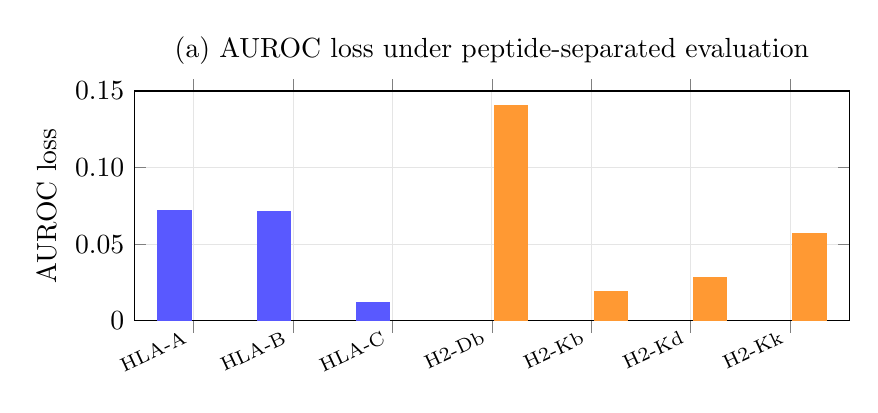
\begin{tikzpicture}
\begin{axis}[
    width=0.88\linewidth,
    height=4.5cm,
    ybar,
    bar width=12pt,
    title={(a) AUROC loss under peptide-separated evaluation},
    ymin=0,ymax=0.15,
    ytick={0,0.05,0.10,0.15},
    yticklabels={0,0.05,0.10,0.15},
    symbolic x coords={HLA-A,HLA-B,HLA-C,H2-Db,H2-Kb,H2-Kd,H2-Kk},
    xtick={HLA-A,HLA-B,HLA-C,H2-Db,H2-Kb,H2-Kd,H2-Kk},
    xticklabels={HLA-A,HLA-B,HLA-C,H2-Db,H2-Kb,H2-Kd,H2-Kk},
    x tick label style={rotate=25,anchor=east,font=\scriptsize},
    ylabel={AUROC loss},
    grid=major,
    grid style={gray!20}
]
\addplot+[fill=blue!65,draw=blue!65] coordinates {(HLA-A,0.0718) (HLA-B,0.0712) (HLA-C,0.0122)};
\addplot+[fill=orange!80,draw=orange!80] coordinates {(H2-Db,0.1404) (H2-Kb,0.0192) (H2-Kd,0.0284) (H2-Kk,0.0571)};
\end{axis}
\end{tikzpicture}

\vspace{0.35cm}

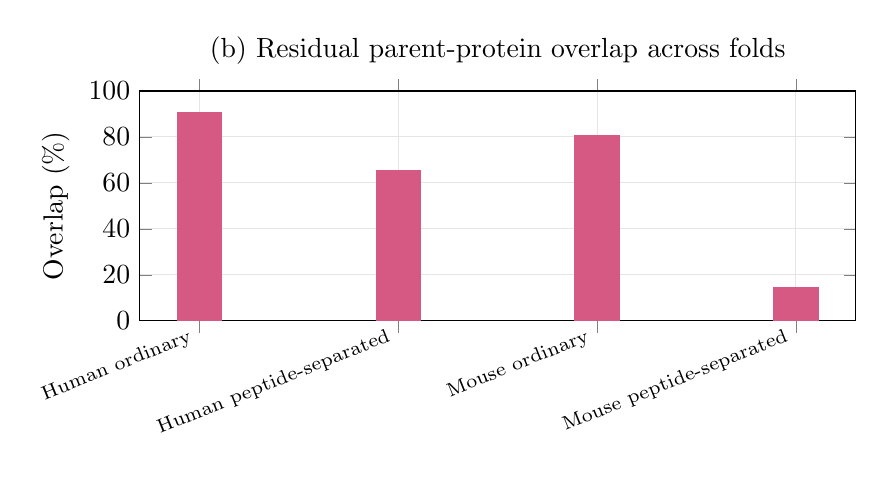
\begin{tikzpicture}
\begin{axis}[
    width=0.88\linewidth,
    height=4.5cm,
    ybar,
    bar width=16pt,
    title={(b) Residual parent-protein overlap across folds},
    ymin=0,ymax=100,
    symbolic x coords={Human matched,Human global,Mouse matched,Mouse global},
    xtick=data,
    xticklabels={Human ordinary,Human peptide-separated,Mouse ordinary,Mouse peptide-separated},
    x tick label style={rotate=22,anchor=east,font=\scriptsize},
    ylabel={Overlap (\%)},
    grid=major,
    grid style={gray!20}
]
\addplot+[fill=purple!65,draw=purple!65] coordinates {(Human matched,90.64) (Human global,65.26) (Mouse matched,80.69) (Mouse global,14.37)};
\end{axis}
\end{tikzpicture}
\caption{Generalization diagnostics using the same pooled evaluation rows. (a) Mean AUROC loss, ordinary minus peptide-separated cross-validation, by HLA gene group or H2 restriction; positive values indicate lower performance when held-out peptide sequences are absent from fitting. (b) Mean fraction of unique held-out parent proteins also observed during fitting; nonzero values quantify residual protein overlap.}
\label{fig:appendix-gap}
\end{figure*}

\clearpage
\refstepcounter{section}
\begin{table*}[!t]
\raggedright
{\large\bfseries \thesection.\ Detailed Model Comparisons When Held-out Peptides Are Absent from All Fitting Combinations\par}
\vspace{0.4\baselineskip}
\centering
\caption{Selected paired AUROC comparisons between models evaluated on the same tissue--MHC combinations and peptide-separated folds. Peptide pairs connected directly or indirectly by a shared sequence are assigned to the same fold. Differences are calculated as the first model minus the second; intervals are based on 10,000 resamples of complete tissue--MHC combinations, and \(q\) values are adjusted within each species--metric family using the Benjamini--Hochberg procedure.}
\label{tab:appendix-strict-paired}
\fontsize{7.5}{8.5}\selectfont
\setlength{\tabcolsep}{1pt}
\begin{tabular}{@{}>{\raggedright\arraybackslash}p{4.15cm}
                   rr
                   >{\centering\arraybackslash}p{1.8cm}
                   >{\centering\arraybackslash}p{2.0cm}
                   >{\centering\arraybackslash}p{1.4cm}@{}}
\toprule
Comparison & Mean & Median & \shortstack{Higher/tied/\\lower} & 95\% CI & Adjusted \(q\) \\
\midrule
\multicolumn{6}{@{}l}{\textit{Human}} \\
TissuePMHC $-$ shared peptide encoder with combination-specific outputs & +0.0091 & +0.0095 & 118/0/39 & [0.0067, 0.0116] & $2.27\times10^{-11}$ \\
TissuePMHC $-$ unguided two-view neural network & +0.0097 & +0.0081 & 122/0/35 & [0.0076, 0.0119] & $1.36\times10^{-14}$ \\
TissuePMHC $-$ guided two-view neural network & +0.0010 & -0.0008 & 76/1/80 & [-0.0008, 0.0029] & 0.442 \\
TissuePMHC $-$ BLOSUM62 random forest & +0.0440 & -- & 149/0/8 & [0.0392, 0.0489] & $3.43\times10^{-26}$ \\
TissuePMHC $-$ one-hot logistic regression & +0.0525 & -- & 157/0/0 & [0.0479, 0.0571] & $8.14\times10^{-27}$ \\
Guided two-view neural network $-$ unguided two-view neural network & +0.0087 & -- & 144/0/13 & [0.0074, 0.0100] & $3.02\times10^{-23}$ \\
Guided two-view neural network $-$ shared peptide encoder with combination-specific outputs & +0.0081 & -- & 123/0/34 & [0.0058, 0.0103] & $3.30\times10^{-11}$ \\
\bottomrule
\end{tabular}
\end{table*}

\begin{table*}[t]
\ContinuedFloat
\centering
\caption[]{Selected paired AUROC comparisons under peptide-separated cross-validation (continued).}
\fontsize{7.5}{8.5}\selectfont
\setlength{\tabcolsep}{1pt}
\begin{tabular}{@{}>{\raggedright\arraybackslash}p{4.15cm}
                   rr
                   >{\centering\arraybackslash}p{1.8cm}
                   >{\centering\arraybackslash}p{2.0cm}
                   >{\centering\arraybackslash}p{1.4cm}@{}}
\toprule
Comparison & Mean & Median & \shortstack{Higher/tied/\\lower} & 95\% CI & Adjusted \(q\) \\
\midrule
\multicolumn{6}{@{}l}{\textit{Mouse}} \\
Mixture of shared modules with combination-specific gates $-$ dual branch with auxiliary supervision & -0.0060 & -0.0057 & 10/0/14 & [-0.0138, 0.0017] & 0.320 \\
Mixture of shared modules with combination-specific gates $-$ BLOSUM62 random forest & +0.0023 & +0.0039 & 14/0/10 & [-0.0050, 0.0092] & 0.611 \\
Mixture of shared modules with combination-specific gates $-$ dual branch without auxiliary supervision & -0.0026 & -0.0022 & 11/0/13 & [-0.0104, 0.0050] & 0.643 \\
Mixture of shared modules with combination-specific gates $-$ one-hot logistic regression & +0.0194 & +0.0206 & 20/0/4 & [0.0119, 0.0264] & $3.81\times10^{-4}$ \\
Mixture of shared modules with combination-specific gates $-$ shared peptide encoder with combination-specific outputs & -0.0008 & -0.0018 & 10/0/14 & [-0.0061, 0.0050] & 0.611 \\
Dual branch with auxiliary supervision $-$ dual branch without auxiliary supervision & +0.0034 & +0.0031 & 21/0/3 & [0.0023, 0.0047] & $2.36\times10^{-5}$ \\
\bottomrule
\end{tabular}
\end{table*}

\begin{table*}[t]
\centering
\caption{Stability across independent training runs and the benefit of averaging their predictions under peptide-separated cross-validation. Peptide-linked groups are kept intact when the folds are formed. Gain is the AUROC obtained after averaging predictions minus the mean AUROC of the separate runs.}
\label{tab:appendix-strict-seeds}
\footnotesize
\setlength{\tabcolsep}{2pt}
\begin{tabularx}{\textwidth}{@{}>{\raggedright\arraybackslash}p{1.05cm}
                                  >{\raggedright\arraybackslash}X
                                  >{\centering\arraybackslash}p{1.45cm}
                                  >{\centering\arraybackslash}p{1.25cm}
                                  >{\centering\arraybackslash}p{1.4cm}
                                  >{\centering\arraybackslash}p{1.15cm}@{}}
\toprule
Species & Model & Mean run & Across-run standard deviation & Averaged predictions & Gain \\
\midrule
Human & One-hot logistic regression & 0.7127 & 0.0000 & 0.7127 & 0.0000 \\
Human & BLOSUM62 random forest & 0.7193 & 0.0006 & 0.7212 & +0.0019 \\
Human & Shared peptide encoder with combination-specific outputs & 0.7313 & 0.0043 & 0.7561 & +0.0248 \\
Human & Unguided two-view neural network & 0.7394 & 0.0043 & 0.7555 & +0.0161 \\
Human & Guided two-view neural network & 0.7503 & 0.0038 & 0.7642 & +0.0139 \\
Human & TissuePMHC & 0.7505 & 0.0007 & 0.7652 & +0.0147 \\
Mouse & One-hot logistic regression & 0.7335 & 0.0000 & 0.7335 & 0.0000 \\
Mouse & BLOSUM62 random forest & 0.7491 & 0.0012 & 0.7507 & +0.0016 \\
Mouse & Shared peptide encoder with combination-specific outputs & 0.7327 & 0.0031 & 0.7538 & +0.0211 \\
Mouse & Dual branch without auxiliary supervision & 0.7381 & 0.0031 & 0.7556 & +0.0175 \\
Mouse & Dual branch with auxiliary supervision & 0.7422 & 0.0028 & 0.7590 & +0.0167 \\
Mouse & Mixture of shared modules with combination-specific gates & 0.7211 & 0.0027 & 0.7529 & +0.0318 \\
\bottomrule
\end{tabularx}
\end{table*}

\clearpage
\refstepcounter{section}
\begin{table*}[!t]
\raggedright
{\large\bfseries \thesection.\ Details of Tissue-blind General Presentation Controls\par}
\vspace{0.4\baselineskip}
\begin{minipage}[t]{\columnwidth}
\caption{Sensitivity analysis comparing the NetMHCpan binding-affinity score with its eluted-ligand score. Both rankings are oriented so that larger scores indicate stronger predicted propensity.}
\label{tab:appendix-netmhcpan-el-ba}
\fontsize{7.5}{8.5}\selectfont
\setlength{\tabcolsep}{1.5pt}
\begin{tabularx}{\columnwidth}{@{}l>{\raggedright\arraybackslash}Xccc@{}}
\toprule
Species & Evaluation & Binding AUROC & Presentation AUROC & Difference \\
\midrule
Human & Saved test & 0.6577 & 0.6833 & +0.0256 \\
Human & Complete training pool & 0.6559 & 0.6823 & +0.0264 \\
Mouse & Saved test & 0.6847 & 0.6893 & +0.0046 \\
Mouse & Complete training pool & 0.6778 & 0.6802 & +0.0024 \\
\bottomrule
\end{tabularx}
\end{minipage}

\par\vspace{1.1\baselineskip}
\centering
\caption{Combining tissue-independent peptide--MHC scores with the corresponding tissue-conditioned model score. The combination rule is learned on other folds, and all external scores were generated before this analysis.}
\label{tab:appendix-general-stacking}
\fontsize{8.5}{9.5}\selectfont
\setlength{\tabcolsep}{3pt}
\begin{tabularx}{\textwidth}{>{\raggedright\arraybackslash}p{1.0cm}
                            >{\raggedright\arraybackslash}X
                            >{\raggedright\arraybackslash}Xrr}
\toprule
Species & Protocol & External control & External only & Combined \\
\midrule
Human & saved internal test set & MHCflurry predicted presentation & 0.6851 & 0.8453 \\
Human & saved internal test set & NetMHCpan eluted-ligand score & 0.6833 & 0.8447 \\
Human & Peptide-separated cross-validation & MHCflurry predicted presentation & 0.6867 & 0.7693 \\
Human & Peptide-separated cross-validation & NetMHCpan eluted-ligand score & 0.6740 & 0.7651 \\
Mouse & saved internal test set & MHCflurry predicted presentation & 0.6564 & 0.8565 \\
Mouse & saved internal test set & NetMHCpan eluted-ligand score & 0.6893 & 0.8564 \\
Mouse & Peptide-separated cross-validation & MHCflurry predicted presentation & 0.6464 & 0.7564 \\
Mouse & Peptide-separated cross-validation & NetMHCpan eluted-ligand score & 0.6420 & 0.7534 \\
\bottomrule
\end{tabularx}
\end{table*}
